% Created by tikzDevice version 0.10.1 on 2017-11-06 20:32:20
% !TEX encoding = UTF-8 Unicode
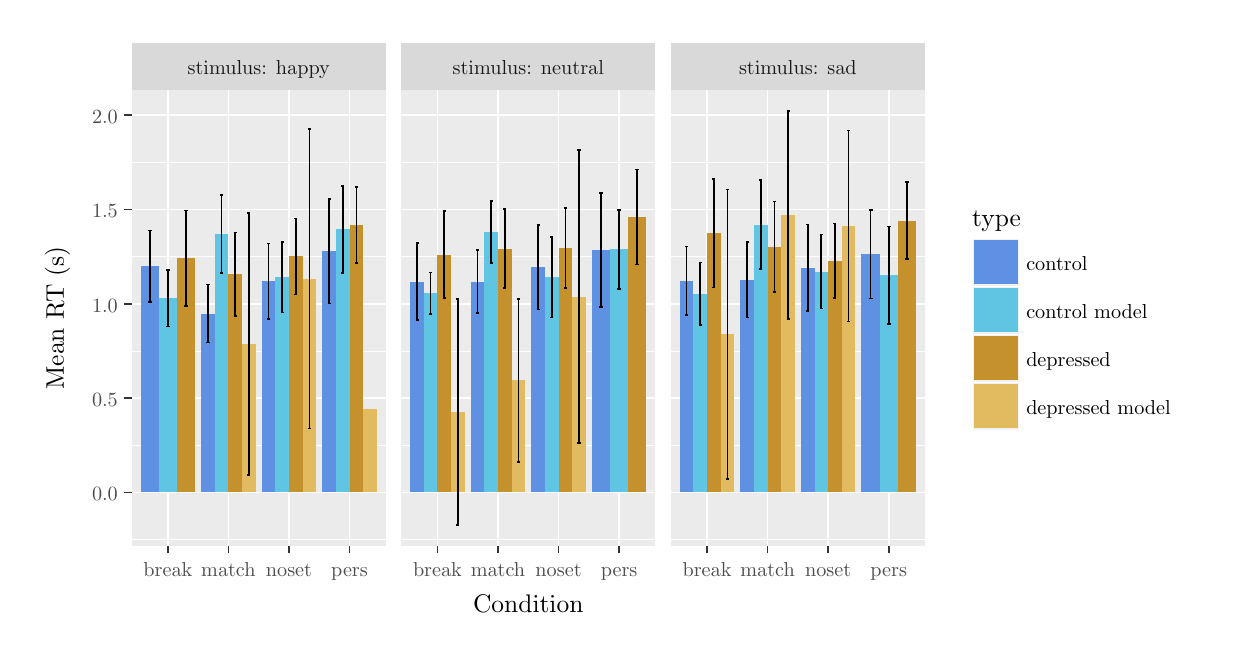
\begin{tikzpicture}[x=1pt,y=1pt]
\definecolor{fillColor}{RGB}{255,255,255}
\path[use as bounding box,fill=fillColor,fill opacity=0.00] (0,0) rectangle (433.62,216.81);
\begin{scope}
\path[clip] (  0.00,  0.00) rectangle (433.62,216.81);
\definecolor{drawColor}{RGB}{255,255,255}
\definecolor{fillColor}{RGB}{255,255,255}

\path[draw=drawColor,line width= 0.6pt,line join=round,line cap=round,fill=fillColor] ( -0.00,  0.00) rectangle (433.62,216.81);
\end{scope}
\begin{scope}
\path[clip] ( 37.53, 29.59) rectangle (129.44,194.25);
\definecolor{fillColor}{gray}{0.92}

\path[fill=fillColor] ( 37.53, 29.59) rectangle (129.44,194.25);
\definecolor{drawColor}{RGB}{255,255,255}

\path[draw=drawColor,line width= 0.3pt,line join=round] ( 37.53, 31.85) --
	(129.44, 31.85);

\path[draw=drawColor,line width= 0.3pt,line join=round] ( 37.53, 65.92) --
	(129.44, 65.92);

\path[draw=drawColor,line width= 0.3pt,line join=round] ( 37.53,100.00) --
	(129.44,100.00);

\path[draw=drawColor,line width= 0.3pt,line join=round] ( 37.53,134.07) --
	(129.44,134.07);

\path[draw=drawColor,line width= 0.3pt,line join=round] ( 37.53,168.15) --
	(129.44,168.15);

\path[draw=drawColor,line width= 0.6pt,line join=round] ( 37.53, 48.88) --
	(129.44, 48.88);

\path[draw=drawColor,line width= 0.6pt,line join=round] ( 37.53, 82.96) --
	(129.44, 82.96);

\path[draw=drawColor,line width= 0.6pt,line join=round] ( 37.53,117.04) --
	(129.44,117.04);

\path[draw=drawColor,line width= 0.6pt,line join=round] ( 37.53,151.11) --
	(129.44,151.11);

\path[draw=drawColor,line width= 0.6pt,line join=round] ( 37.53,185.19) --
	(129.44,185.19);

\path[draw=drawColor,line width= 0.6pt,line join=round] ( 50.66, 29.59) --
	( 50.66,194.25);

\path[draw=drawColor,line width= 0.6pt,line join=round] ( 72.54, 29.59) --
	( 72.54,194.25);

\path[draw=drawColor,line width= 0.6pt,line join=round] ( 94.43, 29.59) --
	( 94.43,194.25);

\path[draw=drawColor,line width= 0.6pt,line join=round] (116.31, 29.59) --
	(116.31,194.25);
\definecolor{fillColor}{RGB}{196,145,45}

\path[fill=fillColor] ( 53.94, 48.88) rectangle ( 60.51,133.46);
\definecolor{fillColor}{RGB}{95,197,226}

\path[fill=fillColor] ( 47.38, 48.88) rectangle ( 53.94,119.07);
\definecolor{fillColor}{RGB}{95,145,226}

\path[fill=fillColor] ( 40.81, 48.88) rectangle ( 47.38,130.60);
\definecolor{fillColor}{RGB}{226,186,95}

\path[fill=fillColor] ( 77.47, 48.88) rectangle ( 82.39,102.53);
\definecolor{fillColor}{RGB}{196,145,45}

\path[fill=fillColor] ( 72.54, 48.88) rectangle ( 77.47,127.67);
\definecolor{fillColor}{RGB}{95,197,226}

\path[fill=fillColor] ( 67.62, 48.88) rectangle ( 72.54,142.25);
\definecolor{fillColor}{RGB}{95,145,226}

\path[fill=fillColor] ( 62.70, 48.88) rectangle ( 67.62,113.49);
\definecolor{fillColor}{RGB}{226,186,95}

\path[fill=fillColor] ( 99.35, 48.88) rectangle (104.27,126.09);
\definecolor{fillColor}{RGB}{196,145,45}

\path[fill=fillColor] ( 94.43, 48.88) rectangle ( 99.35,134.14);
\definecolor{fillColor}{RGB}{95,197,226}

\path[fill=fillColor] ( 89.50, 48.88) rectangle ( 94.43,126.64);
\definecolor{fillColor}{RGB}{95,145,226}

\path[fill=fillColor] ( 84.58, 48.88) rectangle ( 89.50,125.15);
\definecolor{fillColor}{RGB}{226,186,95}

\path[fill=fillColor] (121.23, 48.88) rectangle (126.16, 79.09);
\definecolor{fillColor}{RGB}{196,145,45}

\path[fill=fillColor] (116.31, 48.88) rectangle (121.23,145.46);
\definecolor{fillColor}{RGB}{95,197,226}

\path[fill=fillColor] (111.39, 48.88) rectangle (116.31,143.97);
\definecolor{fillColor}{RGB}{95,145,226}

\path[fill=fillColor] (106.46, 48.88) rectangle (111.39,135.98);
\definecolor{drawColor}{RGB}{0,0,0}

\path[draw=drawColor,line width= 0.6pt,line join=round] ( 56.50,150.70) --
	( 57.96,150.70);

\path[draw=drawColor,line width= 0.6pt,line join=round] ( 57.23,150.70) --
	( 57.23,116.22);

\path[draw=drawColor,line width= 0.6pt,line join=round] ( 56.50,116.22) --
	( 57.96,116.22);

\path[draw=drawColor,line width= 0.6pt,line join=round] ( 49.93,129.29) --
	( 51.39,129.29);

\path[draw=drawColor,line width= 0.6pt,line join=round] ( 50.66,129.29) --
	( 50.66,108.84);

\path[draw=drawColor,line width= 0.6pt,line join=round] ( 49.93,108.84) --
	( 51.39,108.84);

\path[draw=drawColor,line width= 0.6pt,line join=round] ( 43.37,143.48) --
	( 44.83,143.48);

\path[draw=drawColor,line width= 0.6pt,line join=round] ( 44.10,143.48) --
	( 44.10,117.72);

\path[draw=drawColor,line width= 0.6pt,line join=round] ( 43.37,117.72) --
	( 44.83,117.72);

\path[draw=drawColor,line width= 0.6pt,line join=round] ( 79.38,149.89) --
	( 80.48,149.89);

\path[draw=drawColor,line width= 0.6pt,line join=round] ( 79.93,149.89) --
	( 79.93, 55.16);

\path[draw=drawColor,line width= 0.6pt,line join=round] ( 79.38, 55.16) --
	( 80.48, 55.16);

\path[draw=drawColor,line width= 0.6pt,line join=round] ( 74.46,142.80) --
	( 75.55,142.80);

\path[draw=drawColor,line width= 0.6pt,line join=round] ( 75.01,142.80) --
	( 75.01,112.54);

\path[draw=drawColor,line width= 0.6pt,line join=round] ( 74.46,112.54) --
	( 75.55,112.54);

\path[draw=drawColor,line width= 0.6pt,line join=round] ( 69.54,156.40) --
	( 70.63,156.40);

\path[draw=drawColor,line width= 0.6pt,line join=round] ( 70.08,156.40) --
	( 70.08,128.11);

\path[draw=drawColor,line width= 0.6pt,line join=round] ( 69.54,128.11) --
	( 70.63,128.11);

\path[draw=drawColor,line width= 0.6pt,line join=round] ( 64.61,123.99) --
	( 65.71,123.99);

\path[draw=drawColor,line width= 0.6pt,line join=round] ( 65.16,123.99) --
	( 65.16,103.00);

\path[draw=drawColor,line width= 0.6pt,line join=round] ( 64.61,103.00) --
	( 65.71,103.00);

\path[draw=drawColor,line width= 0.6pt,line join=round] (101.27,180.17) --
	(102.36,180.17);

\path[draw=drawColor,line width= 0.6pt,line join=round] (101.81,180.17) --
	(101.81, 72.00);

\path[draw=drawColor,line width= 0.6pt,line join=round] (101.27, 72.00) --
	(102.36, 72.00);

\path[draw=drawColor,line width= 0.6pt,line join=round] ( 96.34,147.91) --
	( 97.44,147.91);

\path[draw=drawColor,line width= 0.6pt,line join=round] ( 96.89,147.91) --
	( 96.89,120.38);

\path[draw=drawColor,line width= 0.6pt,line join=round] ( 96.34,120.38) --
	( 97.44,120.38);

\path[draw=drawColor,line width= 0.6pt,line join=round] ( 91.42,139.43) --
	( 92.51,139.43);

\path[draw=drawColor,line width= 0.6pt,line join=round] ( 91.97,139.43) --
	( 91.97,113.86);

\path[draw=drawColor,line width= 0.6pt,line join=round] ( 91.42,113.86) --
	( 92.51,113.86);

\path[draw=drawColor,line width= 0.6pt,line join=round] ( 86.49,138.85) --
	( 87.59,138.85);

\path[draw=drawColor,line width= 0.6pt,line join=round] ( 87.04,138.85) --
	( 87.04,111.45);

\path[draw=drawColor,line width= 0.6pt,line join=round] ( 86.49,111.45) --
	( 87.59,111.45);

\path[draw=drawColor,line width= 0.6pt,line join=round] (118.22,159.15) --
	(119.32,159.15);

\path[draw=drawColor,line width= 0.6pt,line join=round] (118.77,159.15) --
	(118.77,131.76);

\path[draw=drawColor,line width= 0.6pt,line join=round] (118.22,131.76) --
	(119.32,131.76);

\path[draw=drawColor,line width= 0.6pt,line join=round] (113.30,159.67) --
	(114.40,159.67);

\path[draw=drawColor,line width= 0.6pt,line join=round] (113.85,159.67) --
	(113.85,128.27);

\path[draw=drawColor,line width= 0.6pt,line join=round] (113.30,128.27) --
	(114.40,128.27);

\path[draw=drawColor,line width= 0.6pt,line join=round] (108.38,154.79) --
	(109.47,154.79);

\path[draw=drawColor,line width= 0.6pt,line join=round] (108.92,154.79) --
	(108.92,117.17);

\path[draw=drawColor,line width= 0.6pt,line join=round] (108.38,117.17) --
	(109.47,117.17);
\end{scope}
\begin{scope}
\path[clip] (134.94, 29.59) rectangle (226.85,194.25);
\definecolor{fillColor}{gray}{0.92}

\path[fill=fillColor] (134.94, 29.59) rectangle (226.85,194.25);
\definecolor{drawColor}{RGB}{255,255,255}

\path[draw=drawColor,line width= 0.3pt,line join=round] (134.94, 31.85) --
	(226.85, 31.85);

\path[draw=drawColor,line width= 0.3pt,line join=round] (134.94, 65.92) --
	(226.85, 65.92);

\path[draw=drawColor,line width= 0.3pt,line join=round] (134.94,100.00) --
	(226.85,100.00);

\path[draw=drawColor,line width= 0.3pt,line join=round] (134.94,134.07) --
	(226.85,134.07);

\path[draw=drawColor,line width= 0.3pt,line join=round] (134.94,168.15) --
	(226.85,168.15);

\path[draw=drawColor,line width= 0.6pt,line join=round] (134.94, 48.88) --
	(226.85, 48.88);

\path[draw=drawColor,line width= 0.6pt,line join=round] (134.94, 82.96) --
	(226.85, 82.96);

\path[draw=drawColor,line width= 0.6pt,line join=round] (134.94,117.04) --
	(226.85,117.04);

\path[draw=drawColor,line width= 0.6pt,line join=round] (134.94,151.11) --
	(226.85,151.11);

\path[draw=drawColor,line width= 0.6pt,line join=round] (134.94,185.19) --
	(226.85,185.19);

\path[draw=drawColor,line width= 0.6pt,line join=round] (148.07, 29.59) --
	(148.07,194.25);

\path[draw=drawColor,line width= 0.6pt,line join=round] (169.95, 29.59) --
	(169.95,194.25);

\path[draw=drawColor,line width= 0.6pt,line join=round] (191.83, 29.59) --
	(191.83,194.25);

\path[draw=drawColor,line width= 0.6pt,line join=round] (213.72, 29.59) --
	(213.72,194.25);
\definecolor{fillColor}{RGB}{226,186,95}

\path[fill=fillColor] (152.99, 48.88) rectangle (157.92, 77.97);
\definecolor{fillColor}{RGB}{196,145,45}

\path[fill=fillColor] (148.07, 48.88) rectangle (152.99,134.82);
\definecolor{fillColor}{RGB}{95,197,226}

\path[fill=fillColor] (143.15, 48.88) rectangle (148.07,120.88);
\definecolor{fillColor}{RGB}{95,145,226}

\path[fill=fillColor] (138.22, 48.88) rectangle (143.15,125.08);
\definecolor{fillColor}{RGB}{226,186,95}

\path[fill=fillColor] (174.88, 48.88) rectangle (179.80, 89.36);
\definecolor{fillColor}{RGB}{196,145,45}

\path[fill=fillColor] (169.95, 48.88) rectangle (174.88,136.94);
\definecolor{fillColor}{RGB}{95,197,226}

\path[fill=fillColor] (165.03, 48.88) rectangle (169.95,142.91);
\definecolor{fillColor}{RGB}{95,145,226}

\path[fill=fillColor] (160.10, 48.88) rectangle (165.03,125.01);
\definecolor{fillColor}{RGB}{226,186,95}

\path[fill=fillColor] (196.76, 48.88) rectangle (201.68,119.62);
\definecolor{fillColor}{RGB}{196,145,45}

\path[fill=fillColor] (191.83, 48.88) rectangle (196.76,137.21);
\definecolor{fillColor}{RGB}{95,197,226}

\path[fill=fillColor] (186.91, 48.88) rectangle (191.83,126.54);
\definecolor{fillColor}{RGB}{95,145,226}

\path[fill=fillColor] (181.99, 48.88) rectangle (186.91,130.19);
\definecolor{fillColor}{RGB}{196,145,45}

\path[fill=fillColor] (217.00, 48.88) rectangle (223.56,148.39);
\definecolor{fillColor}{RGB}{95,197,226}

\path[fill=fillColor] (210.43, 48.88) rectangle (217.00,136.69);
\definecolor{fillColor}{RGB}{95,145,226}

\path[fill=fillColor] (203.87, 48.88) rectangle (210.43,136.53);
\definecolor{drawColor}{RGB}{0,0,0}

\path[draw=drawColor,line width= 0.6pt,line join=round] (154.91,118.88) --
	(156.00,118.88);

\path[draw=drawColor,line width= 0.6pt,line join=round] (155.45,118.88) --
	(155.45, 37.07);

\path[draw=drawColor,line width= 0.6pt,line join=round] (154.91, 37.07) --
	(156.00, 37.07);

\path[draw=drawColor,line width= 0.6pt,line join=round] (149.98,150.64) --
	(151.08,150.64);

\path[draw=drawColor,line width= 0.6pt,line join=round] (150.53,150.64) --
	(150.53,119.01);

\path[draw=drawColor,line width= 0.6pt,line join=round] (149.98,119.01) --
	(151.08,119.01);

\path[draw=drawColor,line width= 0.6pt,line join=round] (145.06,128.35) --
	(146.15,128.35);

\path[draw=drawColor,line width= 0.6pt,line join=round] (145.61,128.35) --
	(145.61,113.42);

\path[draw=drawColor,line width= 0.6pt,line join=round] (145.06,113.42) --
	(146.15,113.42);

\path[draw=drawColor,line width= 0.6pt,line join=round] (140.14,139.05) --
	(141.23,139.05);

\path[draw=drawColor,line width= 0.6pt,line join=round] (140.68,139.05) --
	(140.68,111.11);

\path[draw=drawColor,line width= 0.6pt,line join=round] (140.14,111.11) --
	(141.23,111.11);

\path[draw=drawColor,line width= 0.6pt,line join=round] (176.79,118.79) --
	(177.88,118.79);

\path[draw=drawColor,line width= 0.6pt,line join=round] (177.34,118.79) --
	(177.34, 59.93);

\path[draw=drawColor,line width= 0.6pt,line join=round] (176.79, 59.93) --
	(177.88, 59.93);

\path[draw=drawColor,line width= 0.6pt,line join=round] (171.87,151.18) --
	(172.96,151.18);

\path[draw=drawColor,line width= 0.6pt,line join=round] (172.41,151.18) --
	(172.41,122.69);

\path[draw=drawColor,line width= 0.6pt,line join=round] (171.87,122.69) --
	(172.96,122.69);

\path[draw=drawColor,line width= 0.6pt,line join=round] (166.94,154.13) --
	(168.04,154.13);

\path[draw=drawColor,line width= 0.6pt,line join=round] (167.49,154.13) --
	(167.49,131.69);

\path[draw=drawColor,line width= 0.6pt,line join=round] (166.94,131.69) --
	(168.04,131.69);

\path[draw=drawColor,line width= 0.6pt,line join=round] (162.02,136.39) --
	(163.11,136.39);

\path[draw=drawColor,line width= 0.6pt,line join=round] (162.57,136.39) --
	(162.57,113.63);

\path[draw=drawColor,line width= 0.6pt,line join=round] (162.02,113.63) --
	(163.11,113.63);

\path[draw=drawColor,line width= 0.6pt,line join=round] (198.67,172.54) --
	(199.77,172.54);

\path[draw=drawColor,line width= 0.6pt,line join=round] (199.22,172.54) --
	(199.22, 66.70);

\path[draw=drawColor,line width= 0.6pt,line join=round] (198.67, 66.70) --
	(199.77, 66.70);

\path[draw=drawColor,line width= 0.6pt,line join=round] (193.75,151.66) --
	(194.84,151.66);

\path[draw=drawColor,line width= 0.6pt,line join=round] (194.30,151.66) --
	(194.30,122.76);

\path[draw=drawColor,line width= 0.6pt,line join=round] (193.75,122.76) --
	(194.84,122.76);

\path[draw=drawColor,line width= 0.6pt,line join=round] (188.83,141.06) --
	(189.92,141.06);

\path[draw=drawColor,line width= 0.6pt,line join=round] (189.37,141.06) --
	(189.37,112.03);

\path[draw=drawColor,line width= 0.6pt,line join=round] (188.83,112.03) --
	(189.92,112.03);

\path[draw=drawColor,line width= 0.6pt,line join=round] (183.90,145.39) --
	(185.00,145.39);

\path[draw=drawColor,line width= 0.6pt,line join=round] (184.45,145.39) --
	(184.45,114.99);

\path[draw=drawColor,line width= 0.6pt,line join=round] (183.90,114.99) --
	(185.00,114.99);

\path[draw=drawColor,line width= 0.6pt,line join=round] (219.55,165.56) --
	(221.01,165.56);

\path[draw=drawColor,line width= 0.6pt,line join=round] (220.28,165.56) --
	(220.28,131.21);

\path[draw=drawColor,line width= 0.6pt,line join=round] (219.55,131.21) --
	(221.01,131.21);

\path[draw=drawColor,line width= 0.6pt,line join=round] (212.99,150.97) --
	(214.45,150.97);

\path[draw=drawColor,line width= 0.6pt,line join=round] (213.72,150.97) --
	(213.72,122.41);

\path[draw=drawColor,line width= 0.6pt,line join=round] (212.99,122.41) --
	(214.45,122.41);

\path[draw=drawColor,line width= 0.6pt,line join=round] (206.42,157.18) --
	(207.88,157.18);

\path[draw=drawColor,line width= 0.6pt,line join=round] (207.15,157.18) --
	(207.15,115.88);

\path[draw=drawColor,line width= 0.6pt,line join=round] (206.42,115.88) --
	(207.88,115.88);
\end{scope}
\begin{scope}
\path[clip] (232.35, 29.59) rectangle (324.25,194.25);
\definecolor{fillColor}{gray}{0.92}

\path[fill=fillColor] (232.35, 29.59) rectangle (324.25,194.25);
\definecolor{drawColor}{RGB}{255,255,255}

\path[draw=drawColor,line width= 0.3pt,line join=round] (232.35, 31.85) --
	(324.25, 31.85);

\path[draw=drawColor,line width= 0.3pt,line join=round] (232.35, 65.92) --
	(324.25, 65.92);

\path[draw=drawColor,line width= 0.3pt,line join=round] (232.35,100.00) --
	(324.25,100.00);

\path[draw=drawColor,line width= 0.3pt,line join=round] (232.35,134.07) --
	(324.25,134.07);

\path[draw=drawColor,line width= 0.3pt,line join=round] (232.35,168.15) --
	(324.25,168.15);

\path[draw=drawColor,line width= 0.6pt,line join=round] (232.35, 48.88) --
	(324.25, 48.88);

\path[draw=drawColor,line width= 0.6pt,line join=round] (232.35, 82.96) --
	(324.25, 82.96);

\path[draw=drawColor,line width= 0.6pt,line join=round] (232.35,117.04) --
	(324.25,117.04);

\path[draw=drawColor,line width= 0.6pt,line join=round] (232.35,151.11) --
	(324.25,151.11);

\path[draw=drawColor,line width= 0.6pt,line join=round] (232.35,185.19) --
	(324.25,185.19);

\path[draw=drawColor,line width= 0.6pt,line join=round] (245.48, 29.59) --
	(245.48,194.25);

\path[draw=drawColor,line width= 0.6pt,line join=round] (267.36, 29.59) --
	(267.36,194.25);

\path[draw=drawColor,line width= 0.6pt,line join=round] (289.24, 29.59) --
	(289.24,194.25);

\path[draw=drawColor,line width= 0.6pt,line join=round] (311.12, 29.59) --
	(311.12,194.25);
\definecolor{fillColor}{RGB}{226,186,95}

\path[fill=fillColor] (250.40, 48.88) rectangle (255.32,106.07);
\definecolor{fillColor}{RGB}{196,145,45}

\path[fill=fillColor] (245.48, 48.88) rectangle (250.40,142.53);
\definecolor{fillColor}{RGB}{95,197,226}

\path[fill=fillColor] (240.55, 48.88) rectangle (245.48,120.60);
\definecolor{fillColor}{RGB}{95,145,226}

\path[fill=fillColor] (235.63, 48.88) rectangle (240.55,125.42);
\definecolor{fillColor}{RGB}{226,186,95}

\path[fill=fillColor] (272.28, 48.88) rectangle (277.21,149.11);
\definecolor{fillColor}{RGB}{196,145,45}

\path[fill=fillColor] (267.36, 48.88) rectangle (272.28,137.62);
\definecolor{fillColor}{RGB}{95,197,226}

\path[fill=fillColor] (262.43, 48.88) rectangle (267.36,145.62);
\definecolor{fillColor}{RGB}{95,145,226}

\path[fill=fillColor] (257.51, 48.88) rectangle (262.43,125.69);
\definecolor{fillColor}{RGB}{226,186,95}

\path[fill=fillColor] (294.16, 48.88) rectangle (299.09,145.13);
\definecolor{fillColor}{RGB}{196,145,45}

\path[fill=fillColor] (289.24, 48.88) rectangle (294.16,132.58);
\definecolor{fillColor}{RGB}{95,197,226}

\path[fill=fillColor] (284.32, 48.88) rectangle (289.24,128.68);
\definecolor{fillColor}{RGB}{95,145,226}

\path[fill=fillColor] (279.39, 48.88) rectangle (284.32,129.99);
\definecolor{fillColor}{RGB}{196,145,45}

\path[fill=fillColor] (314.41, 48.88) rectangle (320.97,147.09);
\definecolor{fillColor}{RGB}{95,197,226}

\path[fill=fillColor] (307.84, 48.88) rectangle (314.41,127.37);
\definecolor{fillColor}{RGB}{95,145,226}

\path[fill=fillColor] (301.28, 48.88) rectangle (307.84,134.96);
\definecolor{drawColor}{RGB}{0,0,0}

\path[draw=drawColor,line width= 0.6pt,line join=round] (252.31,158.38) --
	(253.41,158.38);

\path[draw=drawColor,line width= 0.6pt,line join=round] (252.86,158.38) --
	(252.86, 53.76);

\path[draw=drawColor,line width= 0.6pt,line join=round] (252.31, 53.76) --
	(253.41, 53.76);

\path[draw=drawColor,line width= 0.6pt,line join=round] (247.39,162.15) --
	(248.48,162.15);

\path[draw=drawColor,line width= 0.6pt,line join=round] (247.94,162.15) --
	(247.94,122.90);

\path[draw=drawColor,line width= 0.6pt,line join=round] (247.39,122.90) --
	(248.48,122.90);

\path[draw=drawColor,line width= 0.6pt,line join=round] (242.47,131.95) --
	(243.56,131.95);

\path[draw=drawColor,line width= 0.6pt,line join=round] (243.01,131.95) --
	(243.01,109.25);

\path[draw=drawColor,line width= 0.6pt,line join=round] (242.47,109.25) --
	(243.56,109.25);

\path[draw=drawColor,line width= 0.6pt,line join=round] (237.54,137.75) --
	(238.64,137.75);

\path[draw=drawColor,line width= 0.6pt,line join=round] (238.09,137.75) --
	(238.09,113.08);

\path[draw=drawColor,line width= 0.6pt,line join=round] (237.54,113.08) --
	(238.64,113.08);

\path[draw=drawColor,line width= 0.6pt,line join=round] (274.20,186.76) --
	(275.29,186.76);

\path[draw=drawColor,line width= 0.6pt,line join=round] (274.74,186.76) --
	(274.74,111.46);

\path[draw=drawColor,line width= 0.6pt,line join=round] (274.20,111.46) --
	(275.29,111.46);

\path[draw=drawColor,line width= 0.6pt,line join=round] (269.27,154.04) --
	(270.37,154.04);

\path[draw=drawColor,line width= 0.6pt,line join=round] (269.82,154.04) --
	(269.82,121.19);

\path[draw=drawColor,line width= 0.6pt,line join=round] (269.27,121.19) --
	(270.37,121.19);

\path[draw=drawColor,line width= 0.6pt,line join=round] (264.35,161.65) --
	(265.44,161.65);

\path[draw=drawColor,line width= 0.6pt,line join=round] (264.90,161.65) --
	(264.90,129.58);

\path[draw=drawColor,line width= 0.6pt,line join=round] (264.35,129.58) --
	(265.44,129.58);

\path[draw=drawColor,line width= 0.6pt,line join=round] (259.43,139.25) --
	(260.52,139.25);

\path[draw=drawColor,line width= 0.6pt,line join=round] (259.97,139.25) --
	(259.97,112.13);

\path[draw=drawColor,line width= 0.6pt,line join=round] (259.43,112.13) --
	(260.52,112.13);

\path[draw=drawColor,line width= 0.6pt,line join=round] (296.08,179.64) --
	(297.17,179.64);

\path[draw=drawColor,line width= 0.6pt,line join=round] (296.63,179.64) --
	(296.63,110.62);

\path[draw=drawColor,line width= 0.6pt,line join=round] (296.08,110.62) --
	(297.17,110.62);

\path[draw=drawColor,line width= 0.6pt,line join=round] (291.16,146.00) --
	(292.25,146.00);

\path[draw=drawColor,line width= 0.6pt,line join=round] (291.70,146.00) --
	(291.70,119.15);

\path[draw=drawColor,line width= 0.6pt,line join=round] (291.16,119.15) --
	(292.25,119.15);

\path[draw=drawColor,line width= 0.6pt,line join=round] (286.23,142.03) --
	(287.33,142.03);

\path[draw=drawColor,line width= 0.6pt,line join=round] (286.78,142.03) --
	(286.78,115.34);

\path[draw=drawColor,line width= 0.6pt,line join=round] (286.23,115.34) --
	(287.33,115.34);

\path[draw=drawColor,line width= 0.6pt,line join=round] (281.31,145.66) --
	(282.40,145.66);

\path[draw=drawColor,line width= 0.6pt,line join=round] (281.86,145.66) --
	(281.86,114.31);

\path[draw=drawColor,line width= 0.6pt,line join=round] (281.31,114.31) --
	(282.40,114.31);

\path[draw=drawColor,line width= 0.6pt,line join=round] (316.96,161.06) --
	(318.42,161.06);

\path[draw=drawColor,line width= 0.6pt,line join=round] (317.69,161.06) --
	(317.69,133.12);

\path[draw=drawColor,line width= 0.6pt,line join=round] (316.96,133.12) --
	(318.42,133.12);

\path[draw=drawColor,line width= 0.6pt,line join=round] (310.39,145.02) --
	(311.85,145.02);

\path[draw=drawColor,line width= 0.6pt,line join=round] (311.12,145.02) --
	(311.12,109.71);

\path[draw=drawColor,line width= 0.6pt,line join=round] (310.39,109.71) --
	(311.85,109.71);

\path[draw=drawColor,line width= 0.6pt,line join=round] (303.83,150.98) --
	(305.29,150.98);

\path[draw=drawColor,line width= 0.6pt,line join=round] (304.56,150.98) --
	(304.56,118.94);

\path[draw=drawColor,line width= 0.6pt,line join=round] (303.83,118.94) --
	(305.29,118.94);
\end{scope}
\begin{scope}
\path[clip] ( 37.53,194.25) rectangle (129.44,211.31);
\definecolor{fillColor}{gray}{0.85}

\path[fill=fillColor] ( 37.53,194.25) rectangle (129.44,211.31);
\definecolor{drawColor}{gray}{0.10}

\node[text=drawColor,anchor=base,inner sep=0pt, outer sep=0pt, scale=  0.73] at ( 83.49,199.75) {stimulus: happy};
\end{scope}
\begin{scope}
\path[clip] (134.94,194.25) rectangle (226.85,211.31);
\definecolor{fillColor}{gray}{0.85}

\path[fill=fillColor] (134.94,194.25) rectangle (226.85,211.31);
\definecolor{drawColor}{gray}{0.10}

\node[text=drawColor,anchor=base,inner sep=0pt, outer sep=0pt, scale=  0.73] at (180.89,199.75) {stimulus: neutral};
\end{scope}
\begin{scope}
\path[clip] (232.35,194.25) rectangle (324.25,211.31);
\definecolor{fillColor}{gray}{0.85}

\path[fill=fillColor] (232.35,194.25) rectangle (324.25,211.31);
\definecolor{drawColor}{gray}{0.10}

\node[text=drawColor,anchor=base,inner sep=0pt, outer sep=0pt, scale=  0.73] at (278.30,199.75) {stimulus: sad};
\end{scope}
\begin{scope}
\path[clip] (  0.00,  0.00) rectangle (433.62,216.81);
\definecolor{drawColor}{gray}{0.20}

\path[draw=drawColor,line width= 0.6pt,line join=round] ( 50.66, 26.84) --
	( 50.66, 29.59);

\path[draw=drawColor,line width= 0.6pt,line join=round] ( 72.54, 26.84) --
	( 72.54, 29.59);

\path[draw=drawColor,line width= 0.6pt,line join=round] ( 94.43, 26.84) --
	( 94.43, 29.59);

\path[draw=drawColor,line width= 0.6pt,line join=round] (116.31, 26.84) --
	(116.31, 29.59);
\end{scope}
\begin{scope}
\path[clip] (  0.00,  0.00) rectangle (433.62,216.81);
\definecolor{drawColor}{gray}{0.30}

\node[text=drawColor,anchor=base,inner sep=0pt, outer sep=0pt, scale=  0.73] at ( 50.66, 18.58) {break};

\node[text=drawColor,anchor=base,inner sep=0pt, outer sep=0pt, scale=  0.73] at ( 72.54, 18.58) {match};

\node[text=drawColor,anchor=base,inner sep=0pt, outer sep=0pt, scale=  0.73] at ( 94.43, 18.58) {noset};

\node[text=drawColor,anchor=base,inner sep=0pt, outer sep=0pt, scale=  0.73] at (116.31, 18.58) {pers};
\end{scope}
\begin{scope}
\path[clip] (  0.00,  0.00) rectangle (433.62,216.81);
\definecolor{drawColor}{gray}{0.20}

\path[draw=drawColor,line width= 0.6pt,line join=round] (148.07, 26.84) --
	(148.07, 29.59);

\path[draw=drawColor,line width= 0.6pt,line join=round] (169.95, 26.84) --
	(169.95, 29.59);

\path[draw=drawColor,line width= 0.6pt,line join=round] (191.83, 26.84) --
	(191.83, 29.59);

\path[draw=drawColor,line width= 0.6pt,line join=round] (213.72, 26.84) --
	(213.72, 29.59);
\end{scope}
\begin{scope}
\path[clip] (  0.00,  0.00) rectangle (433.62,216.81);
\definecolor{drawColor}{gray}{0.30}

\node[text=drawColor,anchor=base,inner sep=0pt, outer sep=0pt, scale=  0.73] at (148.07, 18.58) {break};

\node[text=drawColor,anchor=base,inner sep=0pt, outer sep=0pt, scale=  0.73] at (169.95, 18.58) {match};

\node[text=drawColor,anchor=base,inner sep=0pt, outer sep=0pt, scale=  0.73] at (191.83, 18.58) {noset};

\node[text=drawColor,anchor=base,inner sep=0pt, outer sep=0pt, scale=  0.73] at (213.72, 18.58) {pers};
\end{scope}
\begin{scope}
\path[clip] (  0.00,  0.00) rectangle (433.62,216.81);
\definecolor{drawColor}{gray}{0.20}

\path[draw=drawColor,line width= 0.6pt,line join=round] (245.48, 26.84) --
	(245.48, 29.59);

\path[draw=drawColor,line width= 0.6pt,line join=round] (267.36, 26.84) --
	(267.36, 29.59);

\path[draw=drawColor,line width= 0.6pt,line join=round] (289.24, 26.84) --
	(289.24, 29.59);

\path[draw=drawColor,line width= 0.6pt,line join=round] (311.12, 26.84) --
	(311.12, 29.59);
\end{scope}
\begin{scope}
\path[clip] (  0.00,  0.00) rectangle (433.62,216.81);
\definecolor{drawColor}{gray}{0.30}

\node[text=drawColor,anchor=base,inner sep=0pt, outer sep=0pt, scale=  0.73] at (245.48, 18.58) {break};

\node[text=drawColor,anchor=base,inner sep=0pt, outer sep=0pt, scale=  0.73] at (267.36, 18.58) {match};

\node[text=drawColor,anchor=base,inner sep=0pt, outer sep=0pt, scale=  0.73] at (289.24, 18.58) {noset};

\node[text=drawColor,anchor=base,inner sep=0pt, outer sep=0pt, scale=  0.73] at (311.12, 18.58) {pers};
\end{scope}
\begin{scope}
\path[clip] (  0.00,  0.00) rectangle (433.62,216.81);
\definecolor{drawColor}{gray}{0.30}

\node[text=drawColor,anchor=base east,inner sep=0pt, outer sep=0pt, scale=  0.73] at ( 32.58, 45.85) {0.0};

\node[text=drawColor,anchor=base east,inner sep=0pt, outer sep=0pt, scale=  0.73] at ( 32.58, 79.93) {0.5};

\node[text=drawColor,anchor=base east,inner sep=0pt, outer sep=0pt, scale=  0.73] at ( 32.58,114.01) {1.0};

\node[text=drawColor,anchor=base east,inner sep=0pt, outer sep=0pt, scale=  0.73] at ( 32.58,148.08) {1.5};

\node[text=drawColor,anchor=base east,inner sep=0pt, outer sep=0pt, scale=  0.73] at ( 32.58,182.16) {2.0};
\end{scope}
\begin{scope}
\path[clip] (  0.00,  0.00) rectangle (433.62,216.81);
\definecolor{drawColor}{gray}{0.20}

\path[draw=drawColor,line width= 0.6pt,line join=round] ( 34.78, 48.88) --
	( 37.53, 48.88);

\path[draw=drawColor,line width= 0.6pt,line join=round] ( 34.78, 82.96) --
	( 37.53, 82.96);

\path[draw=drawColor,line width= 0.6pt,line join=round] ( 34.78,117.04) --
	( 37.53,117.04);

\path[draw=drawColor,line width= 0.6pt,line join=round] ( 34.78,151.11) --
	( 37.53,151.11);

\path[draw=drawColor,line width= 0.6pt,line join=round] ( 34.78,185.19) --
	( 37.53,185.19);
\end{scope}
\begin{scope}
\path[clip] (  0.00,  0.00) rectangle (433.62,216.81);
\definecolor{drawColor}{RGB}{0,0,0}

\node[text=drawColor,anchor=base,inner sep=0pt, outer sep=0pt, scale=  0.92] at (180.89,  5.50) {Condition};
\end{scope}
\begin{scope}
\path[clip] (  0.00,  0.00) rectangle (433.62,216.81);
\definecolor{drawColor}{RGB}{0,0,0}

\node[text=drawColor,rotate= 90.00,anchor=base,inner sep=0pt, outer sep=0pt, scale=  0.92] at ( 13.08,111.92) {Mean RT (s)};
\end{scope}
\begin{scope}
\path[clip] (  0.00,  0.00) rectangle (433.62,216.81);
\definecolor{fillColor}{RGB}{255,255,255}

\path[fill=fillColor] (335.63, 65.58) rectangle (428.12,158.25);
\end{scope}
\begin{scope}
\path[clip] (  0.00,  0.00) rectangle (433.62,216.81);
\definecolor{drawColor}{RGB}{0,0,0}

\node[text=drawColor,anchor=base west,inner sep=0pt, outer sep=0pt, scale=  0.92] at (341.32,144.99) {type};
\end{scope}
\begin{scope}
\path[clip] (  0.00,  0.00) rectangle (433.62,216.81);
\definecolor{drawColor}{RGB}{255,255,255}
\definecolor{fillColor}{gray}{0.95}

\path[draw=drawColor,line width= 0.6pt,line join=round,line cap=round,fill=fillColor] (341.32,123.31) rectangle (358.67,140.65);
\end{scope}
\begin{scope}
\path[clip] (  0.00,  0.00) rectangle (433.62,216.81);
\definecolor{fillColor}{RGB}{95,145,226}

\path[fill=fillColor] (342.04,124.02) rectangle (357.96,139.94);
\end{scope}
\begin{scope}
\path[clip] (  0.00,  0.00) rectangle (433.62,216.81);
\definecolor{drawColor}{RGB}{255,255,255}
\definecolor{fillColor}{gray}{0.95}

\path[draw=drawColor,line width= 0.6pt,line join=round,line cap=round,fill=fillColor] (341.32,105.96) rectangle (358.67,123.31);
\end{scope}
\begin{scope}
\path[clip] (  0.00,  0.00) rectangle (433.62,216.81);
\definecolor{fillColor}{RGB}{95,197,226}

\path[fill=fillColor] (342.04,106.67) rectangle (357.96,122.60);
\end{scope}
\begin{scope}
\path[clip] (  0.00,  0.00) rectangle (433.62,216.81);
\definecolor{drawColor}{RGB}{255,255,255}
\definecolor{fillColor}{gray}{0.95}

\path[draw=drawColor,line width= 0.6pt,line join=round,line cap=round,fill=fillColor] (341.32, 88.62) rectangle (358.67,105.96);
\end{scope}
\begin{scope}
\path[clip] (  0.00,  0.00) rectangle (433.62,216.81);
\definecolor{fillColor}{RGB}{196,145,45}

\path[fill=fillColor] (342.04, 89.33) rectangle (357.96,105.25);
\end{scope}
\begin{scope}
\path[clip] (  0.00,  0.00) rectangle (433.62,216.81);
\definecolor{drawColor}{RGB}{255,255,255}
\definecolor{fillColor}{gray}{0.95}

\path[draw=drawColor,line width= 0.6pt,line join=round,line cap=round,fill=fillColor] (341.32, 71.27) rectangle (358.67, 88.62);
\end{scope}
\begin{scope}
\path[clip] (  0.00,  0.00) rectangle (433.62,216.81);
\definecolor{fillColor}{RGB}{226,186,95}

\path[fill=fillColor] (342.04, 71.98) rectangle (357.96, 87.91);
\end{scope}
\begin{scope}
\path[clip] (  0.00,  0.00) rectangle (433.62,216.81);
\definecolor{drawColor}{RGB}{0,0,0}

\node[text=drawColor,anchor=base west,inner sep=0pt, outer sep=0pt, scale=  0.73] at (360.84,128.95) {control};
\end{scope}
\begin{scope}
\path[clip] (  0.00,  0.00) rectangle (433.62,216.81);
\definecolor{drawColor}{RGB}{0,0,0}

\node[text=drawColor,anchor=base west,inner sep=0pt, outer sep=0pt, scale=  0.73] at (360.84,111.60) {control model};
\end{scope}
\begin{scope}
\path[clip] (  0.00,  0.00) rectangle (433.62,216.81);
\definecolor{drawColor}{RGB}{0,0,0}

\node[text=drawColor,anchor=base west,inner sep=0pt, outer sep=0pt, scale=  0.73] at (360.84, 94.26) {depressed};
\end{scope}
\begin{scope}
\path[clip] (  0.00,  0.00) rectangle (433.62,216.81);
\definecolor{drawColor}{RGB}{0,0,0}

\node[text=drawColor,anchor=base west,inner sep=0pt, outer sep=0pt, scale=  0.73] at (360.84, 76.91) {depressed model};
\end{scope}
\end{tikzpicture}
